% -*- Mode:TeX -*-

%% IMPORTANT: The official thesis specifications are available at:
%%            http://libraries.mit.edu/archives/thesis-specs/
%%
%%            Please verify your thesis' formatting and copyright
%%            assignment before submission.  If you notice any
%%            discrepancies between these templates and the 
%%            MIT Libraries' specs, please let us know
%%            by e-mailing thesis@mit.edu

%% The documentclass options along with the pagestyle can be used to generate
%% a technical report, a draft copy, or a regular thesis.  You may need to
%% re-specify the pagestyle after you \include  cover.tex.  For more
%% information, see the first few lines of mitthesis.cls. 

%\documentclass[12pt,vi,twoside]{mitthesis}
%%
%%  If you want your thesis copyright to you instead of MIT, use the
%%  ``vi'' option, as above.
%%
%\documentclass[12pt,twoside,leftblank]{mitthesis}
%%
%% If you want blank pages before new chapters to be labelled ``This
%% Page Intentionally Left Blank'', use the ``leftblank'' option, as
%% above. 

\documentclass[12pt,twoside]{mitthesis}
\usepackage{lgrind}
%% These have been added at the request of the MIT Libraries, because
%% some PDF conversions mess up the ligatures.  -LB, 1/22/2014
\usepackage{cmap}
\usepackage[T1]{fontenc}

%% Custom macros
\usepackage{macros}

\pagestyle{plain}

%% This bit allows you to either specify only the files which you wish to
%% process, or `all' to process all files which you \include.
%% Krishna Sethuraman (1990).

\typein [\files]{Enter file names to process, (chap1,chap2 ...), or `all' to
process all files:}
\def\all{all}
\ifx\files\all \typeout{Including all files.} \else \typeout{Including only \files.} \includeonly{\files} \fi

\begin{document}

% -*-latex-*-
% 
% For questions, comments, concerns or complaints:
% thesis@mit.edu
% 
%
% $Log: cover.tex,v $
% Revision 1.8  2008/05/13 15:02:15  jdreed
% Degree month is June, not May.  Added note about prevdegrees.
% Arthur Smith's title updated
%
% Revision 1.7  2001/02/08 18:53:16  boojum
% changed some \newpages to \cleardoublepages
%
% Revision 1.6  1999/10/21 14:49:31  boojum
% changed comment referring to documentstyle
%
% Revision 1.5  1999/10/21 14:39:04  boojum
% *** empty log message ***
%
% Revision 1.4  1997/04/18  17:54:10  othomas
% added page numbers on abstract and cover, and made 1 abstract
% page the default rather than 2.  (anne hunter tells me this
% is the new institute standard.)
%
% Revision 1.4  1997/04/18  17:54:10  othomas
% added page numbers on abstract and cover, and made 1 abstract
% page the default rather than 2.  (anne hunter tells me this
% is the new institute standard.)
%
% Revision 1.3  93/05/17  17:06:29  starflt
% Added acknowledgements section (suggested by tompalka)
% 
% Revision 1.2  92/04/22  13:13:13  epeisach
% Fixes for 1991 course 6 requirements
% Phrase "and to grant others the right to do so" has been added to 
% permission clause
% Second copy of abstract is not counted as separate pages so numbering works
% out
% 
% Revision 1.1  92/04/22  13:08:20  epeisach

% NOTE:
% These templates make an effort to conform to the MIT Thesis specifications,
% however the specifications can change.  We recommend that you verify the
% layout of your title page with your thesis advisor and/or the MIT 
% Libraries before printing your final copy.
\title{Neuro-Bayesian Methods for Realtime Scene Perception}

\author{Austin J. Garrett}
% If you wish to list your previous degrees on the cover page, use the 
% previous degrees command:
%       \prevdegrees{A.A., Harvard University (1985)}
% You can use the \\ command to list multiple previous degrees
%       \prevdegrees{B.S., University of California (1978) \\
%                    S.M., Massachusetts Institute of Technology (1981)}
\department{Department of Electrical Engineering and Computer Science}

% If the thesis is for two degrees simultaneously, list them both
% separated by \and like this:
% \degree{Doctor of Philosophy \and Master of Science}
\degree{Master of Engineering in Electrical Engineering and Computer Science}

% As of the 2007-08 academic year, valid degree months are September, 
% February, or June.  The default is June.
\degreemonth{December}
\degreeyear{2019}
\thesisdate{December 11, 2019}

%% By default, the thesis will be copyrighted to MIT.  If you need to copyright
%% the thesis to yourself, just specify the `vi' documentclass option.  If for
%% some reason you want to exactly specify the copyright notice text, you can
%% use the \copyrightnoticetext command.  
%\copyrightnoticetext{\copyright IBM, 1990.  Do not open till Xmas.}

% If there is more than one supervisor, use the \supervisor command
% once for each.
\supervisor{Vikash Mansinghka}{Research Scientist}

% This is the department committee chairman, not the thesis committee
% chairman.  You should replace this with your Department's Committee
% Chairman.
\chairman{Placeholder}{Chairman, Department Committee on Graduate Theses}

% Make the titlepage based on the above information.  If you need
% something special and can't use the standard form, you can specify
% the exact text of the titlepage yourself.  Put it in a titlepage
% environment and leave blank lines where you want vertical space.
% The spaces will be adjusted to fill the entire page.  The dotted
% lines for the signatures are made with the \signature command.
\maketitle

% The abstractpage environment sets up everything on the page except
% the text itself.  The title and other header material are put at the
% top of the page, and the supervisors are listed at the bottom.  A
% new page is begun both before and after.  Of course, an abstract may
% be more than one page itself.  If you need more control over the
% format of the page, you can use the abstract environment, which puts
% the word "Abstract" at the beginning and single spaces its text.

%% You can either \input (*not* \include) your abstract file, or you can put
%% the text of the abstract directly between the \begin{abstractpage} and
%% \end{abstractpage} commands.

% First copy: start a new page, and save the page number.
\cleardoublepage
% Uncomment the next line if you do NOT want a page number on your
% abstract and acknowledgments pages.
% \pagestyle{empty}
\setcounter{savepage}{\thepage}
\begin{abstractpage}
%% The text of your abstract and nothing else (other than comments) goes here.
%% It will be single-spaced and the rest of the text that is supposed to go on
%% the abstract page will be generated by the abstractpage environment.  This
%% file should be \input (not \include 'd) from cover.tex.

In this thesis, I designed and implemented a compiler which performs
optimizations that reduce the number of low-level floating point operations
necessary for a specific task; this involves the optimization of chains of
floating point operations as well as the implementation of a ``fixed'' point
data type that allows some floating point operations to simulated with integer
arithmetic.  The source language of the compiler is a subset of C, and the
destination language is assembly language for a micro-floating point CPU.  An
instruction-level simulator of the CPU was written to allow testing of the
code.  A series of test pieces of codes was compiled, both with and without
optimization, to determine how effective these optimizations were.

\end{abstractpage}

% Additional copy: start a new page, and reset the page number.  This way,
% the second copy of the abstract is not counted as separate pages.
% Uncomment the next 6 lines if you need two copies of the abstract
% page.
% \setcounter{page}{\thesavepage}
% \begin{abstractpage}
% %% The text of your abstract and nothing else (other than comments) goes here.
%% It will be single-spaced and the rest of the text that is supposed to go on
%% the abstract page will be generated by the abstractpage environment.  This
%% file should be \input (not \include 'd) from cover.tex.

In this thesis, I designed and implemented a compiler which performs
optimizations that reduce the number of low-level floating point operations
necessary for a specific task; this involves the optimization of chains of
floating point operations as well as the implementation of a ``fixed'' point
data type that allows some floating point operations to simulated with integer
arithmetic.  The source language of the compiler is a subset of C, and the
destination language is assembly language for a micro-floating point CPU.  An
instruction-level simulator of the CPU was written to allow testing of the
code.  A series of test pieces of codes was compiled, both with and without
optimization, to determine how effective these optimizations were.

% \end{abstractpage}

\cleardoublepage

%%%%%%%%%%%%%%%%%%%%%%%%%%%%%%%%%%%%%%%%%%%%%%%%%%%%%%%%%%%%%%%%%%%%%%
% -*-latex-*-

% Some departments (e.g. 5) require an additional signature page.  See
% signature.tex for more information and uncomment the following line if
% applicable.
% \include{signature}
\pagestyle{plain}
  % -*- Mode:TeX -*-
%% This file simply contains the commands that actually generate the table of
%% contents and lists of figures and tables.  You can omit any or all of
%% these files by simply taking out the appropriate command.  For more
%% information on these files, see appendix C.3.3 of the LaTeX manual. 

\tableofcontents
\newpage

%% Should contain a brief summary of the backgroud of the problem and/or overall
%% area you are investigating. You should state your particular motivation for
%% working on the present problem in your thesis as well as reasons for how and
%% why your solution(s) will contribute a new work to the field. In other words,
%% you are articulating a gap in current knowledge. Your thesis should be arguable
%% or falsifiable; the statement you make should be able to be challenged. The
%% terms that you use in your thesis should have strong, clear definitions --
%% perhaps not in the thesis statement itself, but in the same paragraph. For
%% example, your readers will want to know what you mean by "optimal",
%% "efficient", or "high performance".
%% 
%% You should be able to explain the central idea of your thesis with one
%% sentence; if that sentence is too complicated to craft, you may have too many
%% distinct ideas. Remember, your thesis is not the place where you solve all
%% problems -- focus on the original work that you are doing, which is distinct
%% form and important to other work being done in your field.

\chapter{Thesis Proposal}

\section{Introduction}

  The past decade has seen a flourishing of highly powerful computer vision
  techniques, due to the success of deep learning techniques accelerated on
  massively parallel hardware.

  Yet the shortcomings of neural techniques have only grown increasingly urgent
  in proportion to their dominance. While these approaches have resulted in the
  amortization of traditionally very difficult and high-dimensional computer
  vision problems, the lack of semantic structuring in their output has led to
  great challenges in their deployment in practical domains where
  interpretability and composability are desperately needed to integrate these
  components into larger frameworks.

  Meanwhile probabilistic techniques offer a more principled approach to modeling
  structured data, and have seen a rapid growth in the collective ecosystem. Such
  environments are desirable for their expressibility, corresponding to the fact
  that they often represent intuitive models of rationality inspired from
  cognitive and neuroscience which increasingly rely on such modeling to explain
  the human reasoning.


  DATASET??

  This part is a highly relevent research goal, due to the undervaluing of
  semantic structuring of information by the neural network community. In
  some sense we are trying to provide a solution to a problem that is not
  fully visible to the community, or at the very least is thought to be
  "too hard" for current techniques. Hard grounding metrics, or at least a
  fuller range of explicitly specified common-sense tasks will go a long
  way in changing the over-skeptical perspective toward Bayesian techniques
  trying to answer this question. Thus, an important part of the thesis
  work will be identifying the gap that exists between types of problems
  that we'd like to solve (common sense reasoning), and how neural networks
  currently fail to address these problems, as well as providing as much of
  a solution as we can in the time available, which we believe will be
  compelling enough to demonstrate the utility of Bayesian methods in
  modern CV pipelines.

\section{Prior and Related Works}

  \subsection{Accelerating Inverse Graphics}

    An alternative perspective on the problem of pose estimation comes from the
    perspective of ``analysis-by-synthesis'', in which a generative model
    allows for MCMC-based inference, integrating a notion of uncertainty and
    robustness into the estimation procedure. Typically to make inference
    efficient, these approaches include some amount of discriminative training
    to amortize the inference procedure with data-driven kernels.
    \textit{Picture} is a probabilistic programming language for scene
    perception that proposed among others, arbitrary blocked Gibbs moves,
    gradient-based proposals, and elliptical slice sampling in order to
    incorporate bottom-up amortization of MCMC \cite{kulkarni2015picture}.
    Jampani et. al. created the \textit{informed sampler}, a mixed inference
    kernel between a trained state-independent discriminator proposal, and a
    local Gaussian metropolis-hastings move \cite{DBLP:journals/corr/JampaniNLG14}.
    There has also been work on directly using neural networks as
    initialization for MCMC. Yildirim et. al. leveraged convolutional neural
    networks to initialize a Markov chain for face processing
    \cite{yildirim2015efficient}. 

  \subsection{Neural Approaches to Pose Estimation}

    Only recently have neural approaches successfully begun to make headway on
    full 6D (3 spatial, 3 rotational) pose estimation for multiple objects.
    These algorithms offer a powerful modeling perspective that can be used as
    an intermediate step for segmentation, bounding box regression, or feature
    extraction. However, they often suffer from the same brittleness and
    lack of insight as deep learning in general.

    \cite{xiang2017posecnn} combines heuristical Hough voting and convolutional
    feature extraction to approach the problem. \cite{DBLP:journals/corr/abs-1809-10790}
    uses a neural network to estimate belief maps of keypoints in 2D image
    coordinates that are fed into a standard perspective-$n$-point (P$n$P)
    algorithm to recover the full 6D pose. It was trained only on synthetic
    data, using domain randomization to generalize to the real world.
    \cite{kundu20183d} uses a render-and-compare based loss inspired by inverse
    graphics methods to train the neural regressor.

  \subsection{Bayesian Inference over Structured Scenes} \label{section:1.2.3}

    Extending from this previous work on inverse graphics, we wish to construct
    generative models that contain richer \textit{semantic information} about
    objects in the scene -- namely human-interpretable information about the
    relations between objects. This can be crucial in reducing the complexity
    of inference by reducing the dimensionality of the parametrization to be
    inferred.

    \subsubsection{Scene Graph Representation}

      \begin{figure}
        \centering
        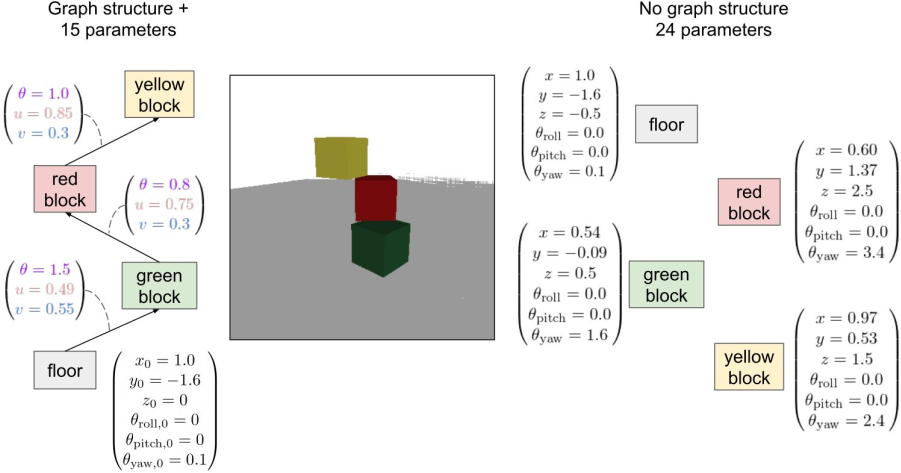
\includegraphics[width=\textwidth]{figures/contact-graph.png}
        \caption{\small
          Two identical representations of three blocks stacked on top of a
          floor in a virtual environment. The right side assumes no semantic
          relational information, with 24 parameters required to specify the
          positions of all the objects in the scene. The left side represents
          semantic information about the relationship between objects, namely
          edges represent an ``on-top of'' relationship. Under this scene
          structure, only 15 parameters are necessary for specifying the same
          scene.\cite{zinberg2019scenegraphs}
        }
        \label{fig:contact-graph}
      \end{figure}

      To encode structural information, we leverage a common computer vision
      representation called a \textit{scene graph}. In this graph, poses are
      represented as transformations from object to object, or from implicit
      world frame to object. Directed edges specify the type of relative pose,
      which encodes information about the way objects are geometrically
      situated. For example, an edge may represent ``contact'', which requires
      specifying a contact plane, a 2D translation, and a single rotational
      DoF.

    \subsubsection{Probabilistic Scene Description Languages}

      \begin{figure}
          \centering
          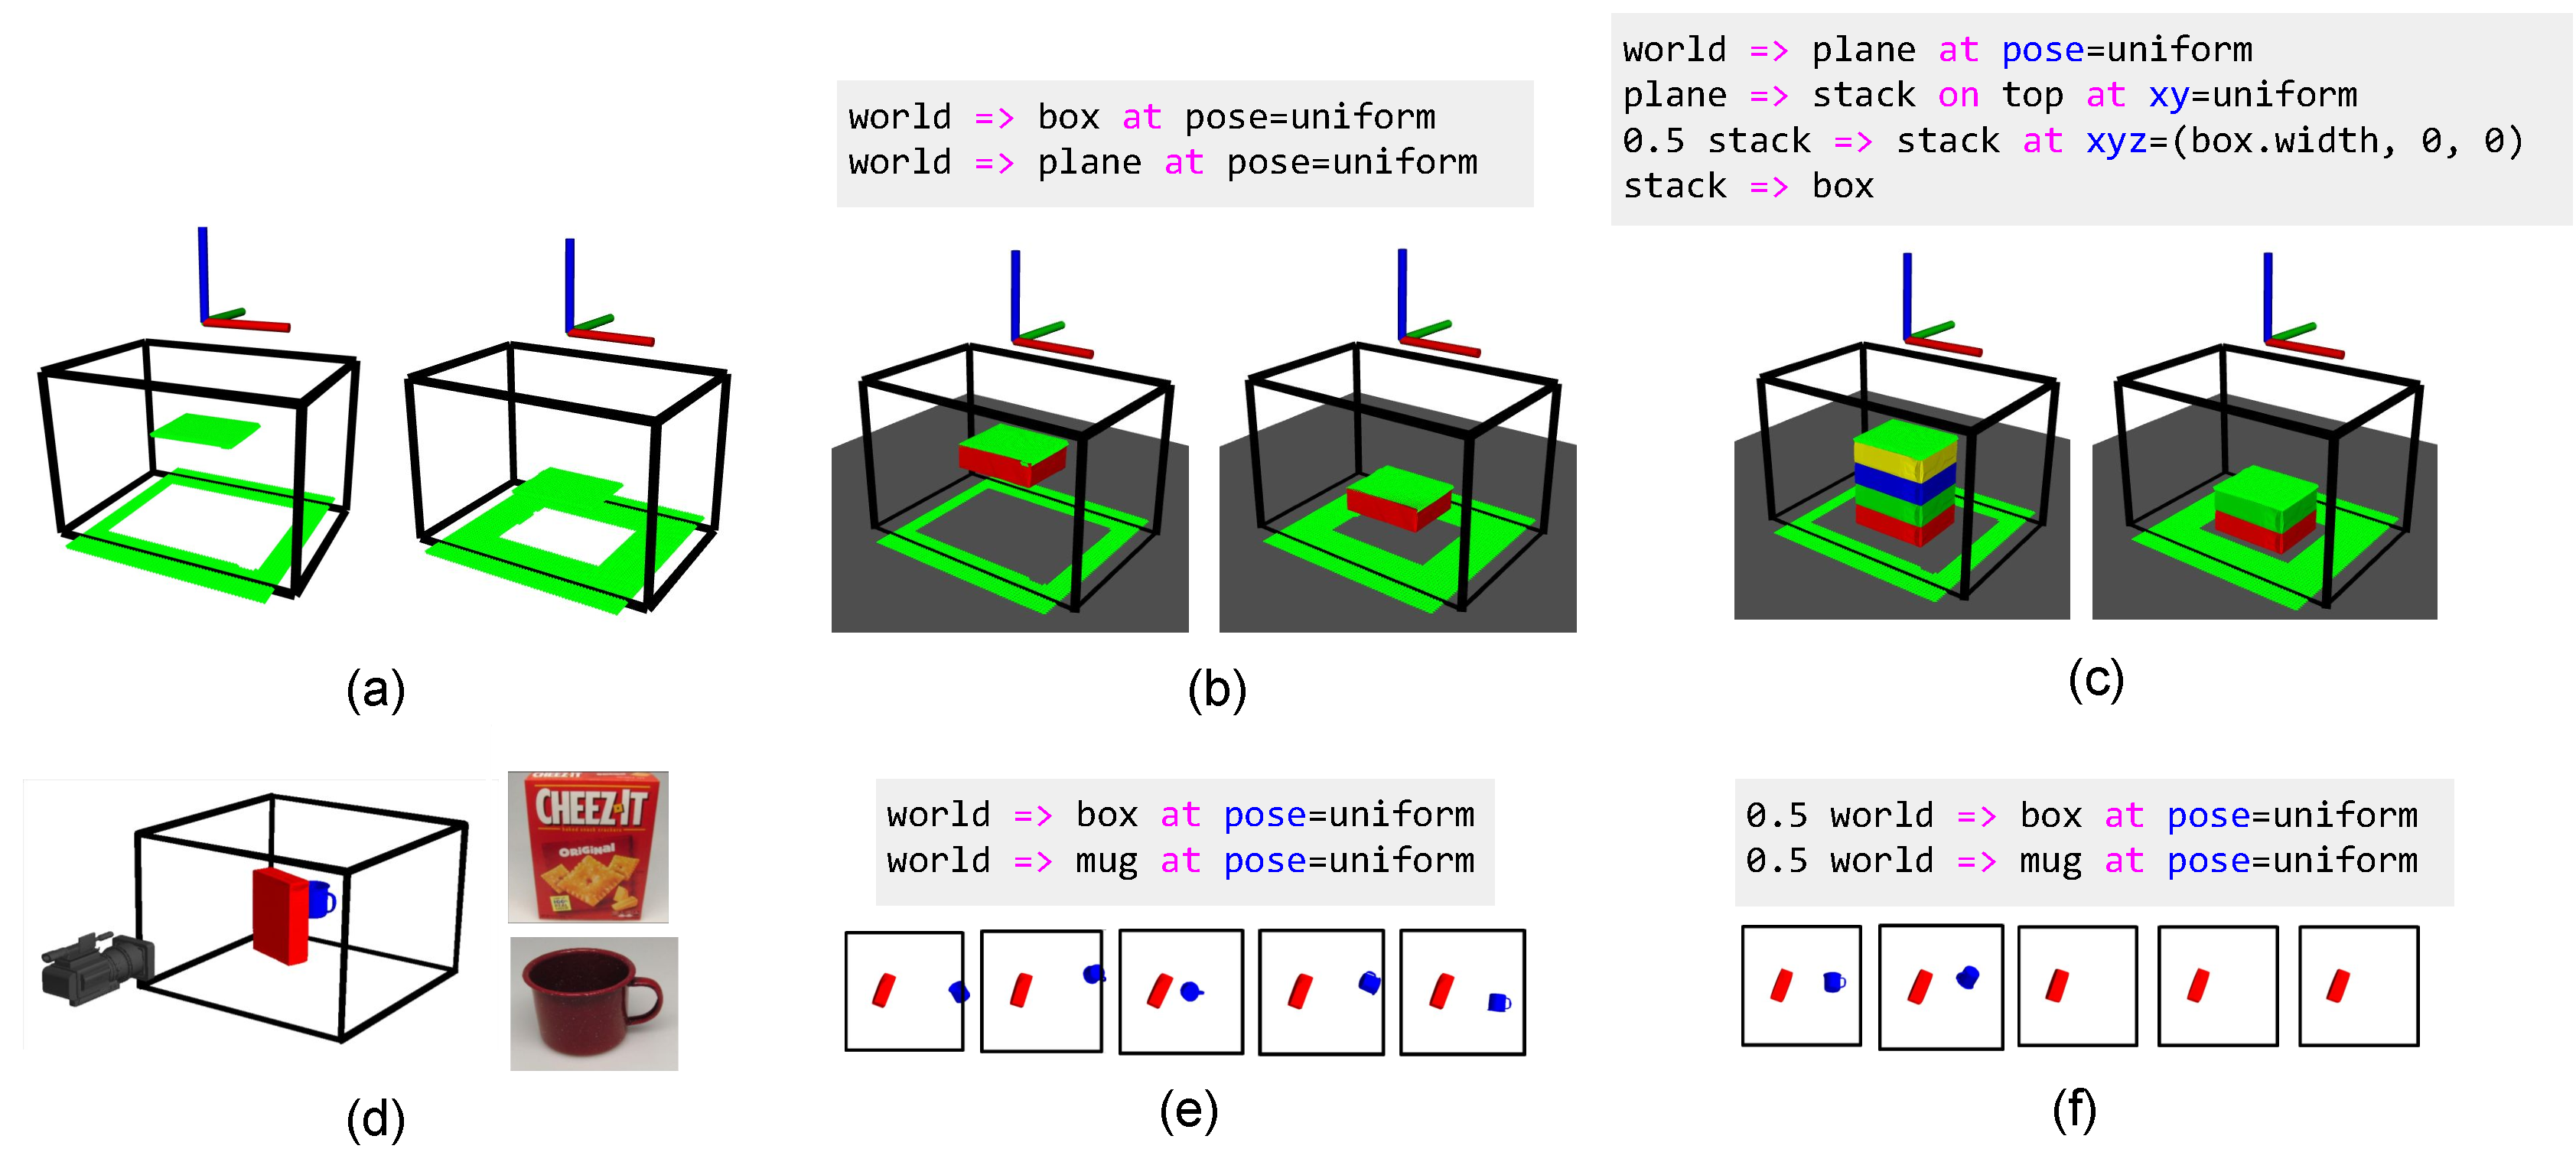
\includegraphics[width=\textwidth]{figures/lafi-fig.pdf}
          \caption{\small
            Two scenarios with prior knowledge specified as programs in our probabilistic scene description language.
            (a) shows two depth measurements made by a depth camera.
            (b) shows a program in which boxes have random poses in 3D space, and the resulting inferred pose of the box.
            (c) shows a program that assumes boxes are in stacks that rest on the floor, and the inferred number of boxes that explain the data for each observation.
            (d) shows another scenario, where a depth camera observes a box that is occluding a mug.
            (e) shows a program that asserts that both objects exist (but at unknown poses).
            The resulting inferences show the mug must exist somewhere behind the box to be consistent with this knowledge and the observation.
            (f) shows a program that allows for either object to not exist, and the resulting joint inferences about the mug's existence and pose.
          }
          \label{fig:results}
      \end{figure}

      It can often be desirable to specify knowledge in a programmatic way. One
      way to define a generative model over a scene graph representation is
      through a probabilistic context free grammar called a \textit{scene
      description language}. Such a language can further increase the
      expressibility of the scene graph concept by adding existential
      uncertainty to the objects themselves. This is encoded by some
      probability over an expansion of the production rules in the PCFG.
      
      Even without the use of data-driven proposals, we can demonstrate how
      this language for uncertain knowledge representation can recover
      common-sense reasoning that naturally combines prior knowledge with
      observation to obtain posteriors with rich structural information.

%% In this subsection, along with an outline of the work that you plan to do -- from
%% the start to the end of your project -- you should also indicate what you think
%% could possibly change as you embark on and continually work on your thesis. In
%% the outline of your work, you might want to describe your methods of data
%% collection, any hardware or software you plan to build or implement, or any
%% algorithms you design. Who you are and what you bring to your work will also
%% help define what you plan to do. Here I quote Professor Neil Spring quite
%% broadly:
%% 
%%   Provide personal insight [to your thesis proposal]. You undoubtedly have a
%%   different way of viewing the world than anyone else, perhaps more theoretical
%%   or practical or empirical or operational. Maybe you think more like a user or
%%   more like a software engineer. [Maybe you had an interesting internship or
%%   spend a summer abroad.] Perhaps your undergraduate minor shapes your
%%   worldview.
%% 
%%   Wherever this project leads you, it's what you bring to the process that
%%   makes it interesting for everyone else. Focus on techniques. Focus on the
%%   methods and how they can be applied to solve a problem. You can make an
%%   exception if conflicating or changing results motivate further analysis.
%%   Often the inputs (workload, applications, processor speeds, network speeds)
%%   will change, and so the results (performace, comparisons) and conclusions
%%   will change with them.
%% 
%% You should also indicate what kind of equipment, facilities, data, or other
%% material you may need for the completion of your work. It is imperative that
%% you provide a timeline or a clear schedule that indicates a plan for your
%% thesis work. In this plan you and your thesis supervisor should come to an
%% agreement on goals for each month of the project including (but not limited to)
%% experiments, data collection, analysis, any refining, drafting of thesis, final
%% results, and revision of thesis. You are welcome to insert a chart with a
%% summary of your goals for each month. Most EECS Master's degree theses are
%% assigned a total number of 360 hours. We ask that you plan accordingly.

\section{Proposed Work}

  \begin{table}[h]
    \begin{tabularx}{\textwidth}{|c|X|}
      \hline
      \textbf{Month} & \textbf{Work to be completed} \\
      \hline
      December & Thesis proposal and ROS-based infrastructure for online particle filtering and associated visualization \\
      \hline
      January  & Experimentation with observational models for modeling neural detections. Writing submission to the RSS conference. \\
      \hline
      February & Refactoring code base and integration of the ROS particle filter and visualization components into Cora. \\
      \hline
      March    & Further integration/experimentation with the neural detector component (training on synthetic data, replacing with alternative architectures, training the neural component with error-correction on inference.) \\
      \hline
      April    & Development of thesis, documentation of work, and writing. \\
      \hline
      May      & Finalization of thesis and final documentation of work and code base. \\
      \hline
    \end{tabularx}
  \end{table}

  \begin{figure}
    \centering
    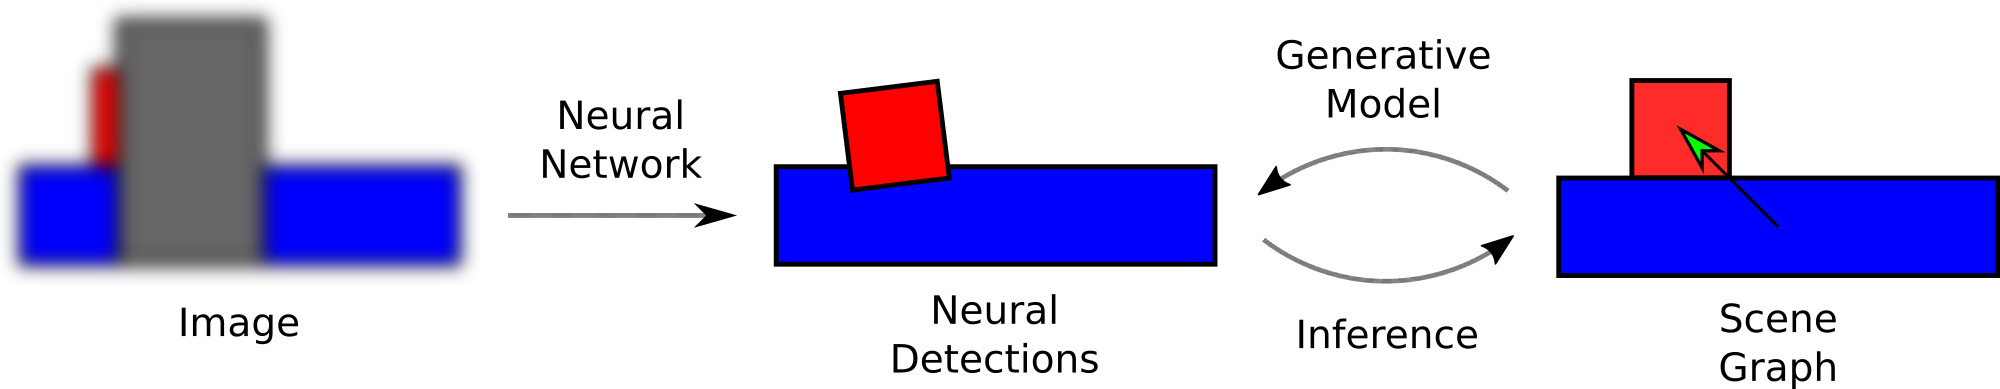
\includegraphics[width=\textwidth]{figures/neural-model.png}
    \caption{\small
      Neural detections can be inaccurate, and violate semantic relations
      between objects (eg. allow for object interpenetration). Given a neural
      detector, we can treat the flat and noisy detections as observations
      under a generative model, given prior structural information about the
      scene. Thus we implicitly model and correct for the failure modes of
      neural detections using uncertain prior structural knowledge. Using
      custom inference kernels, we can potentially recover the network's
      uncertainty, resolve impossible scenarios that violate prior knowledge,
      or even recover qualitative pose relationships like contact (green arrow)
      to enrich neural detections.
    }
    \label{fig:neural-model}
  \end{figure}
  

  \subsection{Neuro-predictive Generative Modeling}

    Modeling a rendering pipeline in a fully Bayesian way suffers from certain
    computational challenges. While guaranteed to converge to a correct
    posterior with unlimited compute time, the non-asymptotic properties of
    MCMC are poorly-understood. Preliminary work in inverse graphics techniques
    applied to structured scenes supports the hypothesis that naive
    analysis-by-synthesis approaches that leverage a full rendering pipeline
    often fail to explore all the modes of the posterior in reasonable time bounds
    \todo[WHO?]

    Concretely, for scene graph $\mathcal{S}$ and continuous parameterization
    $\vec{\nu}_\mathcal{S}$, a rendering-based likelihood relies on modeling
    the image data using a full rendering pipeline $R(\mathcal{S},
    \vec{\nu}_\mathcal{S}) = X$, where $X$ is a rendered image. For robustness,
    the likelihood is modeled not directly on $X$, but on a noisy function of
    the pixel data. The noise is modeled is a mixture of a uniform distribution
    on the range of possible values and a normal distribution with mean
    centered at the true rendered pixel value $R(\mathcal{S},
    \vec{\nu}_\mathcal{S})$ with fixed variance $\sigma^2$, leaving the full
    likelihood on noisy image data $Y$ as
    \begin{equation} \label{eq:1.1}
      p(Y | \mathcal{S}, \vec{\nu}_\mathcal{S}) = \prod_{r=1}^R\prod_{c=1}^C \paren{0.1 \cdot \frac{1}{D} + 0.9 \cdot \mathcal{N}(Y_{r,c}; R(\mathcal{S}, \vec{\nu}_\mathcal{S})_{r,c},\sigma)}
    \end{equation}

    \ref{eq:1.1} is very high-dimensional, making it prone to capture by local
    minima. Neural networks empirically demonstrate strong performance at
    locating strong \textit{maximum a posteriori} estimates in bounded compute
    time. Thus, we may consider combining neural techniques with MCMC to
    improve performance of inference.
    
    One perspective may consider neural networks as amortizations of the
    inverse generative procedure. Consider a neural detector $\phi_\mathcal{S}$
    that outputs poses under a given parametrization $\mathcal{S}$ (often a
    full unconstrained 6D pose), such that ideally $\phi_\mathcal{S}(R(\mathcal{S},
    \vec{\nu}_\mathcal{S})) = \vec{\nu}_\mathcal{S}$. Given image data $Y$, we
    can use the corresponding estimate $\phi_\mathcal{S}(Y)$ as an
    initialization for some MCMC technique.
    
    However, this method is rather unprincipled in that it uses a point
    estimate without uncertainty quantification, thus implicitly relying on
    $\phi_\mathcal{S}$ robustly predicting the mode of the distribution. This
    assumption is not guaranteed, and in fact when neural networks do fail,
    they often fail catastrophically, estimating wildly incorrect poses.
    Furthermore, because it is only a heuristic and not a full proposal
    distribution, it is not obvious how to combine neural detections across
    multiple timesteps into a coherent picture.  The issue fundamentally lies
    in the fact that this approach contains no way to reason about the behavior
    of the bottom-up proposals.  If we wish to robustly use these models, we
    need to leverage information about their behavior.

    Crucially, we can observe that the failure modes of these neural techniques
    are often quite predictable with the use of certain easy to compute
    statistics. When objects are too close or too far away, at strange angles,
    or heavily occluded, the neural detector is much more likely to fail. To
    account for these configurations, we propose instead modeling the neural
    detections as observations to a generative model that attempts to retrieve
    the latent scene graph $\mathcal{S}$ that predicts the detections from the
    neural network $\phi_\mathcal{S}(Y)$.

    A minimal observational model may be a simple mixture between a Gaussian
    and a uniform distribution over the entire space
    \begin{equation} \label{eq:1.2}
      p(\phi_\mathcal{S}(Y) | \mathcal{S}, \vec{\nu}_\mathcal{S}) = \mathcal{N}()
    \end{equation}

    Even such a simple observational model can be sufficient to filter some
    noise from the bottom-up proposal, by roughly modeling that the neural
    network sometimes makes mistakes (although in this case we don't use
    information about whether this is more or less likely at any given time).

  \subsection{Experimentation}

    The first task concrete task is creating the infrastructure sufficient for
    creating a minimal demo. For this we will develop an end-to-end system that
    uses DOPE+Gen+ROS to track a fixed set of objects, integrating prior
    knowledge about temporal consistency of object trajectories via state space
    modeling. For this, we can use a simple particle filter over object
    trajectories. This will help us nail down the end-to-end integration
    aspect, and also serves as the minimal example of ``filtering the output of
    a neural network via prior knowledge''. For simplicity we will initially
    work with an observation model of the form \ref{eq:1.2}. Even with this
    simple model, we hypothesis it is possible to filter spurious neural
    detections using physical assumptions of object persistence and intertial
    trajectories.

    Use the full pipeline to infer scene structure, integrating prior knowledge
    about scene graphs (e.g. contact relationships) as well as temporal
    consistency. This version will assume a static scene graph, but can later
    be adapted into an online algorithm by running the algorithm on the past
    e.g. 10 time steps of data in sliding windows.
    Use the full pipeline with a prior about temporal consistency of scene
    graphs (e.g. scene graphs change relatively infrequently).

    \subsubsection{Reversible Jump MCMC}

      Allowing MH moves between model parametrizations requires special
      mathematical consideration to ensure detailed balance is satisfied.
      \todo[Insert math]


  \subsection{Engineering Infrastructure}

    All of this experimentation requires sophisticated and novel infrastructure 
    for the prototyping of complex custom inference kernels and observational models
    to be applied in realtime 

    \subsubsection{Realtime Particle Filtering}


    \subsubsection{Visualization}

    \todo

    \subsubsection{Cora Project}

    \todo


  \subsection{Extensions}

    If time permits, there are several possible extensions to this work that
    may be considered. One relates \todo

%% You may wish to provide a paragraph or two to reiterate the thesis/main
%% argument of proposed research and possibly to indicate what work may not be
%% addressed due to the time constraints of an MEng thesis.

\chapter{Conclusion}

\todo

\section{Placeholder}

\todo

\appendix
%% This defines the bibliography file (main.bib) and the bibliography style.
%% If you want to create a bibliography file by hand, change the contents of
%% this file to a `thebibliography' environment.  For more information 
%% see section 4.3 of the LaTeX manual.
\begin{singlespace}
\bibliography{main}
\bibliographystyle{plain}
\end{singlespace}

% Chapter 2

@article{green2009reversible,
  title={Reversible jump MCMC},
  author={Green, Peter J and Hastie, David I},
  journal={Genetics},
  volume={155},
  number={3},
  pages={1391--1403},
  year={2009},
  publisher={Citeseer}
}

@inproceedings{Cusumano-Towner:2019:GGP:3314221.3314642,
 author = {Cusumano-Towner, Marco F. and Saad, Feras A. and Lew, Alexander K. and Mansinghka, Vikash K.},
 title = {Gen: A General-purpose Probabilistic Programming System with Programmable Inference},
 booktitle = {Proceedings of the 40th ACM SIGPLAN Conference on Programming Language Design and Implementation},
 series = {PLDI 2019},
 year = {2019},
 isbn = {978-1-4503-6712-7},
 location = {Phoenix, AZ, USA},
 pages = {221--236},
 numpages = {16},
 url = {http://doi.acm.org/10.1145/3314221.3314642},
 doi = {10.1145/3314221.3314642},
 acmid = {3314642},
 publisher = {ACM},
 address = {New York, NY, USA},
 keywords = {Markov chain Monte Carlo, Probabilistic programming, sequential Monte Carlo, variational inference},
}


% Chapter 3

@article{markley2007averaging,
  title={Averaging quaternions},
  author={Markley, F Landis and Cheng, Yang and Crassidis, John L and Oshman, Yaakov},
  journal={Journal of Guidance, Control, and Dynamics},
  volume={30},
  number={4},
  pages={1193--1197},
  year={2007}
}

@INPROCEEDINGS{Ellson03graphvizand,
    author = {John Ellson and Emden R. Gansner and Eleftherios Koutsofios and Stephen C. North and Gordon Woodhull},
    title = {Graphviz and dynagraph – static and dynamic graph drawing tools},
    booktitle = {GRAPH DRAWING SOFTWARE},
    year = {2003},
    pages = {127--148},
    publisher = {Springer-Verlag}
}

\end{document}
